\subsection{Transfer to bearings, ECG, and synthetic cycles}
\label{sec:transfer-main}

\paragraph{Setup reminder.}
Table~\ref{tab:transfer-main} reports whole-curve prolonged residual $R$ after training/searching DenoiseOpt
(\texttt{hybrid\_lstm}, $250$ outer iterations, seed \texttt{1902771841}) on each transfer board
from Section~\ref{sec:transfer-protocol} ($n{=}256$ periods, $L{=}256$).
Columns are: CWRU/MFPT bearing revolutions, MIT-BIH/PTB-XL ECG beats, and synthetic CNC/PMU pilots.
This pilot uses the historical prolonged-$R$ FitCell objective (frozen
\href{https://github.com/reeldemo/reelsynth/blob/main/brand/artifacts/signal_heal_transfer/results_table.json}{results\_table.json});
it is \emph{not} a v10.1 $R_{\mathrm{blend}}$ retag.
Domain-trained Noise2Noise quality scores were not run on these boards
(latency Table~\ref{tab:transfer-latency} reports zero-shot wavetable N2N timing only).
Deep SOTA rows remain \emph{not executed} (Table~\ref{tab:transfer-sota-status}).
Artifacts:
\href{https://github.com/reeldemo/reelsynth/tree/main/brand/artifacts/signal_heal_transfer}{signal\_heal\_transfer}.

\begin{table*}[t]
  \centering
  \caption{Wrap-heal transfer under prolonged residual $R$ (higher better; historical whole-curve score).
    DenoiseOpt trains/searches \texttt{hybrid\_lstm} for $250$ iterations per domain (seed \texttt{1902771841}).
    Boards: CWRU/MFPT bearing revolutions, MIT-BIH/PTB-XL ECG beats, synthetic CNC/PMU pilots
    ($n{=}256$ periods each). Classical board only; domain-trained N2N quality not executed;
    no invented deep-SOTA scores.}
  \label{tab:transfer-main}
  \setlength{\tabcolsep}{2.8pt}
  \begin{tabular}{@{}lrrrrrr@{}}
    \toprule
    Method & CWRU & MFPT & MIT-BIH & PTB-XL & synth CNC & synth PMU \\
    \midrule
    Ours (\texttt{hybrid\_lstm}) & 0.9623 & 0.9411 & 0.9565 & 0.9336 & 0.9918 & 0.9915 \\
    no-bake & 0.8451 & 0.8657 & 0.7495 & 0.7503 & 0.4499 & 0.9356 \\
    endpoint-pin & 0.5054 & 0.5446 & 0.8650 & 0.8569 & 0.4096 & 0.9442 \\
    \texttt{seam\_fir3} & 0.4483 & 0.5726 & 0.7662 & 0.7462 & 0.5344 & 0.9119 \\
    DualCosine & 0.4608 & 0.4830 & 0.4137 & 0.4769 & 0.4943 & 0.8272 \\
    \bottomrule
  \end{tabular}
\end{table*}

\begin{figure*}[t]
  \centering
  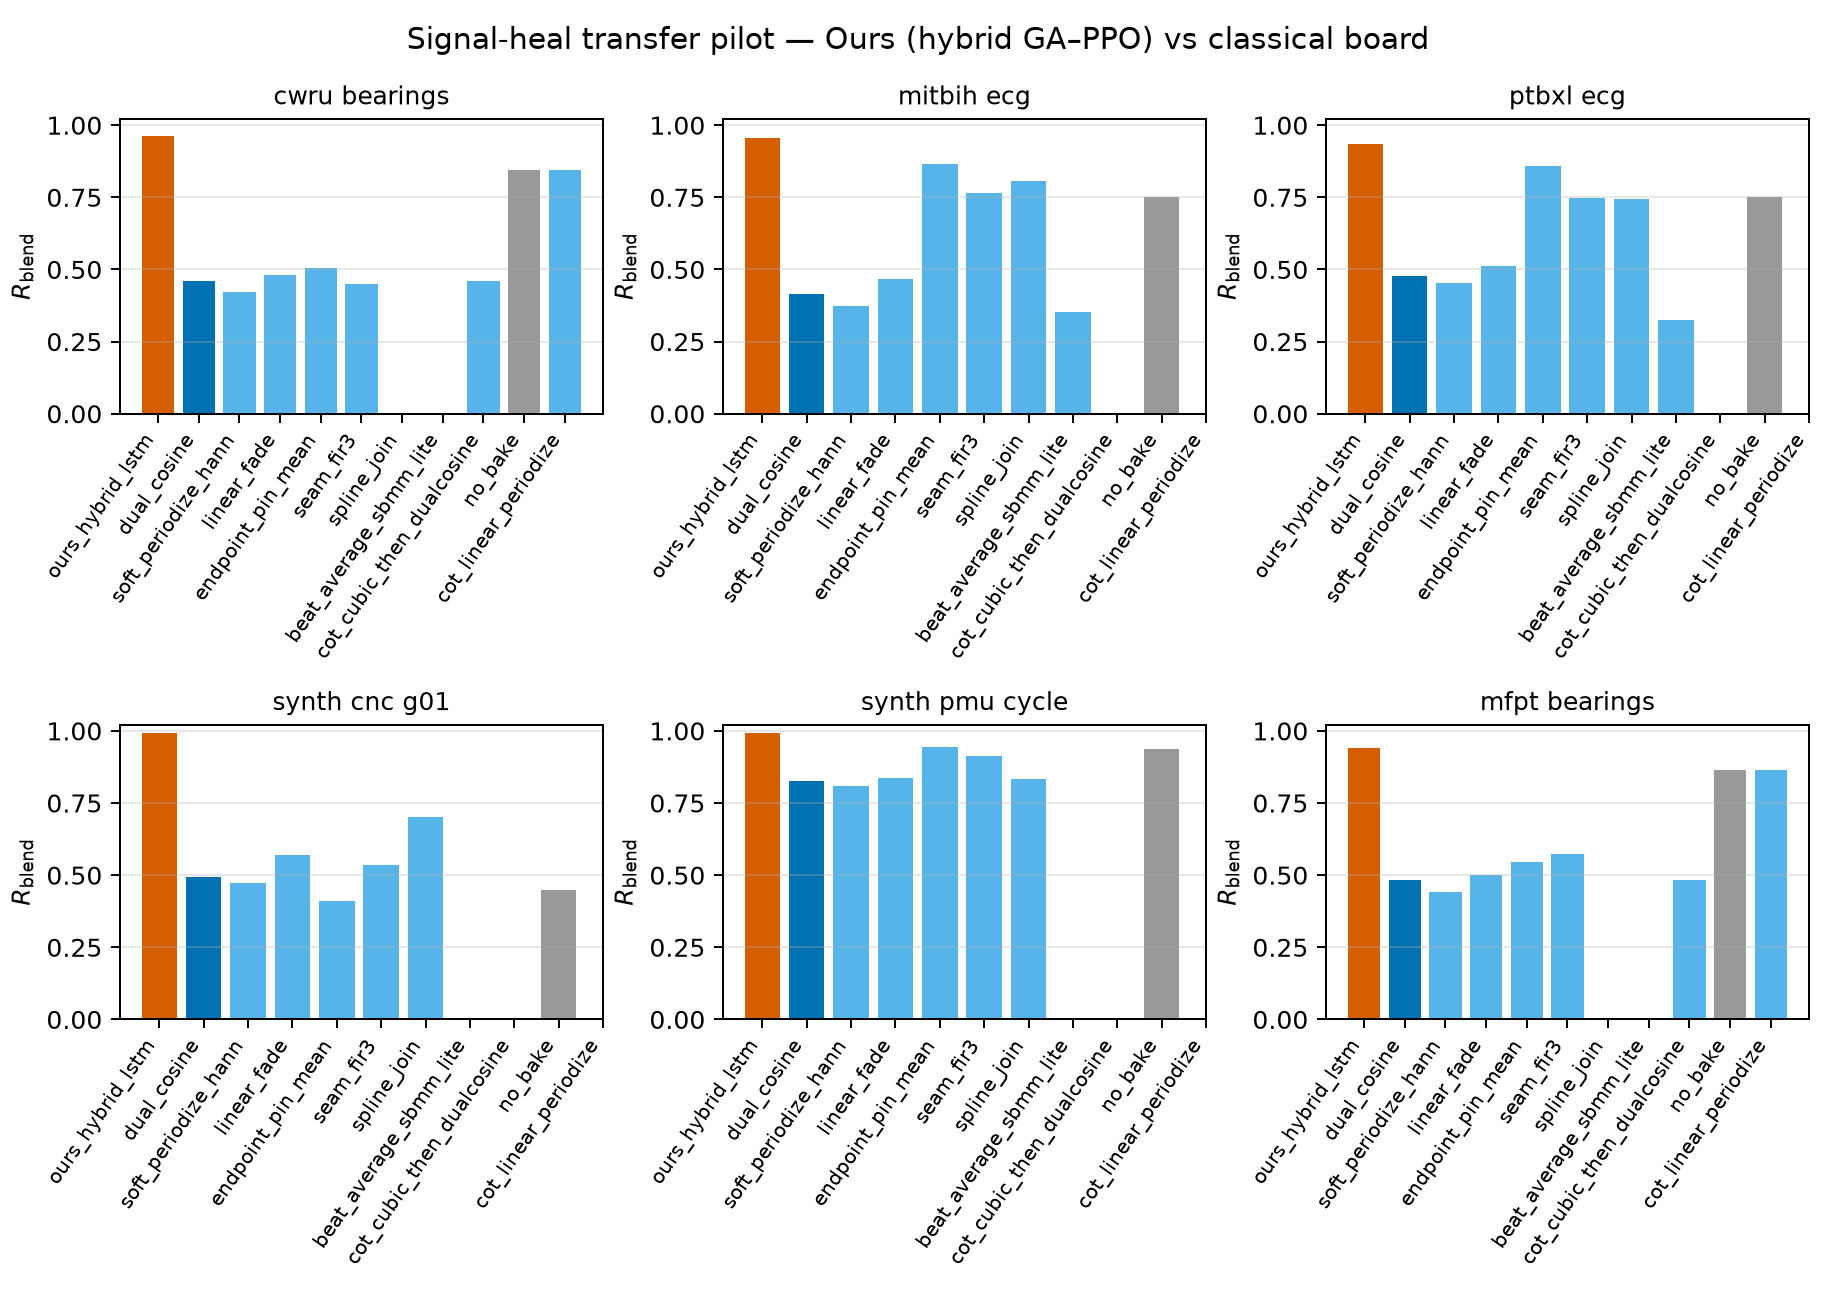
\includegraphics[width=\textwidth,height=0.38\textheight,keepaspectratio]{figures/fig_signal_heal_transfer.png}
  \caption{Transfer classical-board summary (holdout-refit prolonged $R$; grouped bars for Table~\ref{tab:transfer-main}).
    Not a deep-SOTA claim; domain-trained N2N quality not run; see Table~\ref{tab:transfer-sota-status}.}
  \label{fig:signal-heal-transfer-main}
\end{figure*}

\begin{table}[t]
  \centering
  \caption{Deep / real-data transfer status under this residual protocol.
    No invented scores.}
  \label{tab:transfer-sota-status}
  \setlength{\tabcolsep}{3pt}
  \resizebox{\columnwidth}{!}{%
  \begin{tabular}{@{}ll@{}}
    \toprule
    Item & Status \\
    \midrule
    Domain-trained N2N quality & \emph{not executed} (zero-shot WT N2N latency only) \\
    Cycle-GAN (ECG) & \emph{not executed} (no weights under this residual) \\
    BeatDiff & \emph{not executed} \\
    Paderborn KAt deep & \emph{not executed} (registration / multi-GB) \\
    Full PTB-XL corpus & deferred (\texttt{records500} \texttt{*\_hr} subset, $n{=}256$) \\
    Real KIT CNC / IEEE PMU & deferred (login walls; synth pilots ran) \\
    Formal MOS/MUSHRA & deferred (Section~\ref{sec:listening-protocol}) \\
    \bottomrule
  \end{tabular}%
  }
\end{table}

\paragraph{Takeaways.}
Under prolonged $R$, Ours leads every classical-board column in Table~\ref{tab:transfer-main},
including Dual Cosine on every domain.
On CWRU/MFPT, Dual Cosine and fades trail no-bake; Ours clears both by a large margin.
On MIT-BIH and PTB-XL, endpoint-pin is a strong classical ECG row, but Ours still leads.
Synthetic CNC shows the largest classical collapse with Ours near $0.992$.
Domain-trained Noise2Noise quality was not run on these boards
(zero-shot timing in Appendix~\ref{app:supplement}).
Primary claim remains cycle-local wavetable seam restoration.

\subsection{Listening protocol (no formal listening study)}
\label{sec:listening-protocol}

Downloadable WAVs
(\href{https://github.com/reeldemo/reelsynth/tree/main/brand/artifacts/meta_approach_compare/hear_samples}{hear-sample WAVs})
and vibrato spectrograms support informal A/B inspection
(Sections~\ref{sec:vibrato-eval}--\ref{sec:hear-samples}).
Formal MOS / MUSHRA scores were not collected.
Until a formal study runs, perceptual claims remain qualitative and secondary to residual scores.
See Section~\ref{sec:limitations}.
